\documentclass[a4paper, 12pt]{article}

\usepackage[portuguese]{babel}
\usepackage{blindtext}
\usepackage{listings}
\usepackage{mathptmx}
\usepackage{microtype}
\usepackage{enumitem}
\usepackage{amsmath}
\usepackage{index}
\usepackage{fancyhdr}
\usepackage{tikz}
\usepackage{amssymb}
\usepackage{float}
\usepackage{nicematrix}
\usepackage{xcolor}
\usepackage{soulutf8}
\usepackage[hyphens]{url}
\usepackage{bm}
\usetikzlibrary{matrix}
\usetikzlibrary{patterns,decorations.pathreplacing}
\usepackage{graphicx}
\graphicspath{ {./} }

\usepackage[utf8]{inputenc}
\usepackage[T1]{fontenc}
\usepackage{float}
\usepackage{booktabs}
\usepackage{listings}
%\usepackage{listingsutf8}

%--------------------------------------
 
%Portuguese-specific commands
%--------------------------------------
\usepackage[portuguese]{babel}

%% Sets page size and margins
\usepackage[a4paper,top=3cm,bottom=2cm,left=3cm,right=3cm,marginparwidth=1.75cm]{geometry}

%% Useful packages
\usepackage{amsmath}
\usepackage{amsfonts}
\usepackage{graphicx}
\usepackage[colorinlistoftodos]{todonotes}
\usepackage[colorlinks=true, allcolors=black]{hyperref}
\usepackage{caption}
\usepackage{subcaption}
\usepackage{indentfirst}
\usepackage{pgfplots}   % pacote para uso do pgfplots
\usepackage{hyperref} % pacote para inserir links com \url{}
\usepackage{siunitx}
\usepackage{pgfplotstable}
\usepackage{xcolor}



\definecolor{mygrey}{gray}{0.95}
\definecolor{mygreen}{cmyk}{0 1 0.00005 0}
\definecolor{comment}{cmyk}{0.99998 1 0 0}
\definecolor{number}{gray}{0}
\definecolor{string}{cmyk}{0 0.99988 1 0}



\lstdefinestyle{mystyle}{
    backgroundcolor=\color{mygrey},   
    commentstyle=\color{comment},
    keywordstyle=\color{mygreen},
    numberstyle=\tiny\color{number},
    stringstyle=\color{string},
    basicstyle=\ttfamily\footnotesize,
    breakatwhitespace=false,         
    breaklines=true,                 
    captionpos=b,                    
    keepspaces=true,                 
    numbers=left,                    
    numbersep=5pt,                  
    showspaces=false,                
    showstringspaces=false,
    showtabs=false,                  
    tabsize=2,
    language=python,
    literate=
        {á}{{\'a}}1
        {à}{{\`a}}1
        {ã}{{\~a}}1
        {â}{{\^a}}1
        {é}{{\'e}}1
        {ê}{{\^e}}1
        {í}{{\'i}}1
        {ó}{{\'o}}1
        {õ}{{\~o}}1
        {ú}{{\'u}}1
        {ü}{{\"u}}1
        {ç}{{\c{c}}}1
}

\lstset{style=mystyle}

\def\checkmark{\tikz\fill[scale=0.4](0,.35) -- (.25,0) -- (1,.7) -- (.25,.15) -- cycle;} 
\DeclareUnicodeCharacter{2212}{-}
\newcommand*\circled[1]{\tikz[baseline=(char.base)]{
            \node[shape=circle,draw,inner sep=2pt] (char) {#1};}}
\newcommand*\R{\mathbb{R}}
\newcolumntype{C}{>{\centering\let\newline\\\arraybackslash\ $}m{3cm}<{$}}


\begin{document}
\title{\Large{\textbf{Projeto I}}}
\author{
        Gabriel Belém Barbosa \\RA: 234672
}
\date{06 de Novembro de 2021}

\maketitle
\let\cleardoublepage\clearpage
\newpage
\setcounter{page}{2}
\tableofcontents
\newpage
\section{Exercício 1}


\subsection{Algoritmo por partes}
O algoritmo funciona de maneira simples. Primeiramente, uma matriz \verb+G+ com a descrição dada no enunciado é construída, sendo \verb+c+ variado para obter-se as diferentes matrizes desejadas (\verb+c=1+, \verb+c=10+, \verb+c=100+ e \verb+c=1000+ para cada item, respectivamente). Algumas outras variáveis são inicializadas, como o vetor de frações de $\lambda$, e o vetor que armazenará o número de iterações para cada proporção e o número total de iterações, que será fixado em 100 para todos os itens. Algoritmo:
\begin{lstlisting}
c=1;
G=c*diag(1:10);
G(1,1)=1
iterations=zeros(5,1);
scale=[0.1, 0.3, 0.5, 0.75, 1];
num_iter=100;
\end{lstlisting}
Em seguida há um \verb+for+ em \verb+t+ que efetua as iterações para diferentes pontos iniciais. Em cada uma dessas iterações, o ponto inicial para o método, $x_0$, é criado com a função \verb+rand+, que retorna um vetor de dimensão 10 com valores randômicos entre 0 e 1, e então cada entrada de $x_0$ é multiplicada por um inteiro não nulo entre -10 e 10. Em seguida é calculado o gradiente da função em $x_0$, \verb+grad_0+, sendo que $\nabla f(x) =\nabla\left( \frac{1}{2}x^TGx\right)=Gx$, e também a norma do gradiente ao quadrado em $x_0$,  \verb+normgrad_0+. Algoritmo:
\begin{lstlisting}
for t=1:num_iter
    xk_0=rand(10,1);
    for i=1:10
        do
            aux=randi([-10,10]);
        until aux!=0
        xk_0(i)*=aux;
    endfor
    grad_0=G*xk_0;
    normgrad_0=dot(grad_0,grad_0);
\end{lstlisting}
Um novo \verb+for+, desta vez em \verb+i+, que percorre as diferentes frações de $\lambda$, é criado, o contador de iterações \verb+j+ é (re)definido como 0, e as variáveis \verb+xk+,  \verb+grad+ e  \verb+normgrad+ que serão utilizadas no método são (re)definidas como as variáveis encontradas anteriormente para $x_0$. Após isso há um \verb+while+ que institui a condição de parada (que nesse caso é a norma do gradiente ao quadrado do iterando ser menor ou igual que a precisão de máquina, já que a convergência é garantida para esse caso, como visto em aula). Dentro deste \verb+while+ o $\lambda$ do passo exato é calculado, como descrito no método dos gradientes
\[
\lambda=-\frac{\nabla f(x_k)^Td_k}{d_k^TH_f(x_k)d_k}=-\frac{\nabla f(x_k)^T(-\nabla f(x_k))}{(-\nabla f(x_k))^TG(-\nabla f(x_k))}=\frac{||\nabla f(x_k)||^2}{\nabla f(x_k)^TG\nabla f(x_k)}
\]
Então $x_k$ é atualizado, sendo $x_{k+1}$ encontrado como $x_k$ mais uma proporção (\verb+scale(i)+, que é a i-ésima entrada do vetor de frações) de $\lambda$ vezes a direção de menos o vetor gradiente. O gradiente no novo iterando é calculado, assim como sua norma, o número de iterações é atualizado, e o \verb+while+ é finalizado. Ao fim do processo, o número de iterações obtido é somado ao total para aquela fração (\verb+iterations(i)+), e o \verb+for+ em \verb+i+ e em \verb+t+ são finalizados.
\begin{lstlisting}
    for i=1:5
        j=0;
        xk=xk_0;
        grad=grad_0;
        normgrad=normgrad_0;
        while (normgrad>eps)
            lambda=normgrad/(transpose(grad)*G*grad);
            xk-=scale(i)*lambda*grad;
            grad=G*xk;
            normgrad=dot(grad,grad);
            j++;
        endwhile
        iterations(i)+=j;
    endfor
endfor
\end{lstlisting}
Algoritmo completo:
\begin{lstlisting}
c=1;
G=c*diag(1:10);
G(1,1)=1
iterations=zeros(5,1);
scale=[0.1, 0.3, 0.5, 0.75, 1];
num_iter=100;
for t=1:num_iter
    t
    xk_0=rand(10,1);
    for i=1:10
        do
            aux=randi([-10,10]);
        until aux!=0
        xk_0(i)*=aux;
    endfor
    grad_0=G*xk_0;
    normgrad_0=dot(grad_0,grad_0);
    for i=1:5
        j=0;
        xk=xk_0;
        grad=grad_0;
        normgrad=normgrad_0;
        while (normgrad>eps)
            lambda=normgrad/(transpose(grad)*G*grad);
            xk-=scale(i)*lambda*grad;
            grad=G*xk;
            normgrad=dot(grad,grad);
            j++;
        endwhile
        iterations(i)+=j;
    endfor
endfor
\end{lstlisting}
\subsection{Resultados}
\begin{figure}[H]
  \centering
  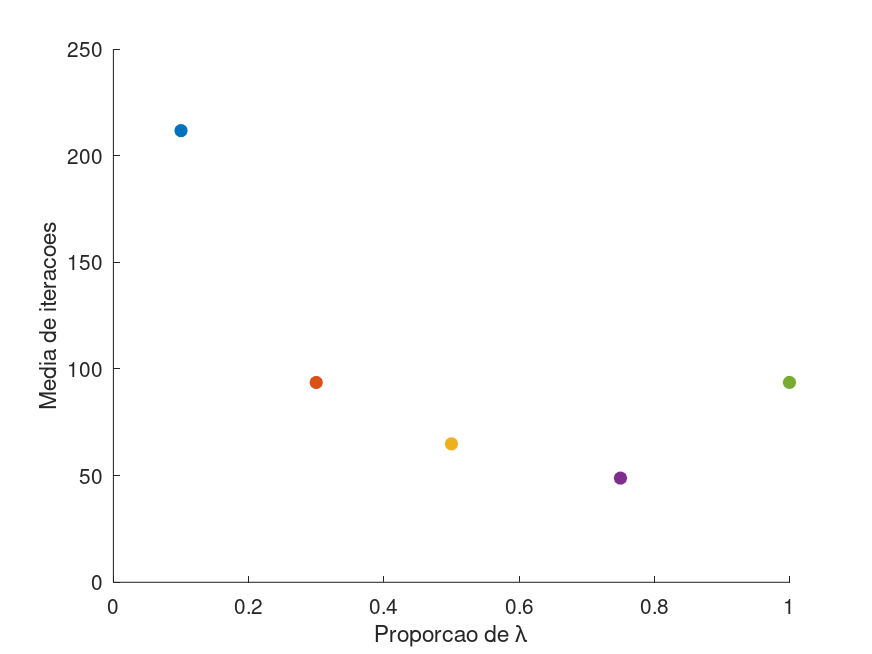
\includegraphics[scale=0.45]{grad.png}
  \caption{G = diag(1, 2, . . . , 10)}
\end{figure}
\begin{figure}[H]
  \centering
  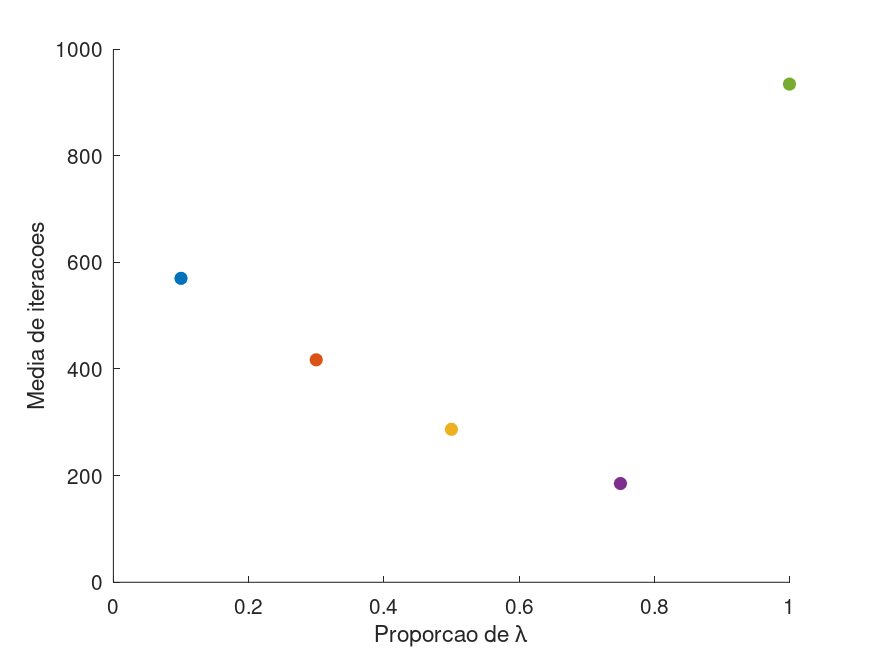
\includegraphics[scale=0.45]{grad10.png}
  \caption{G = diag(1, 20, . . . , 100)}
\end{figure}
\begin{figure}[H]
  \centering
  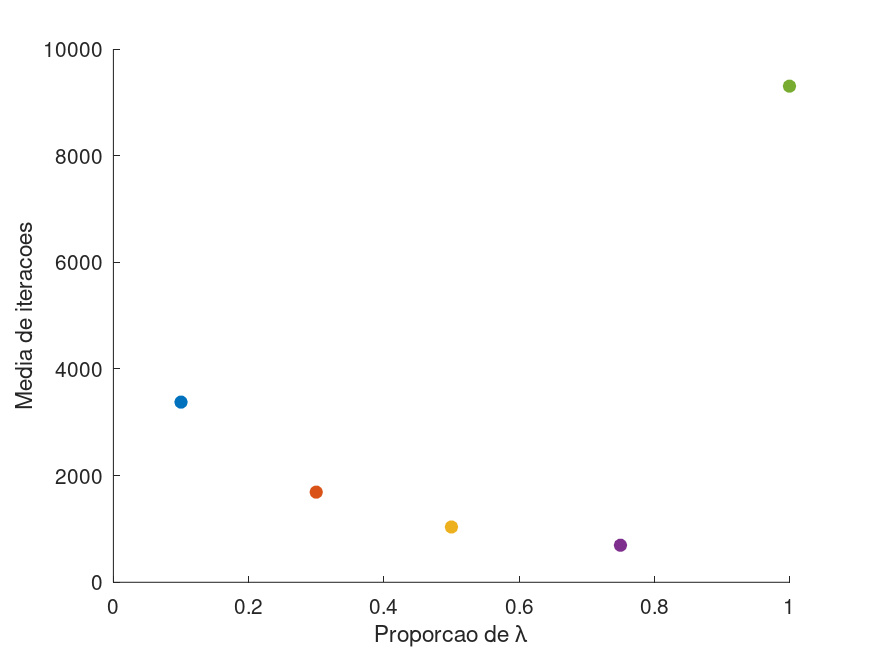
\includegraphics[scale=0.45]{grad100.png}
  \caption{G = diag(1, 200, . . . , 1000)}
\end{figure}
\begin{figure}[H]
  \centering
  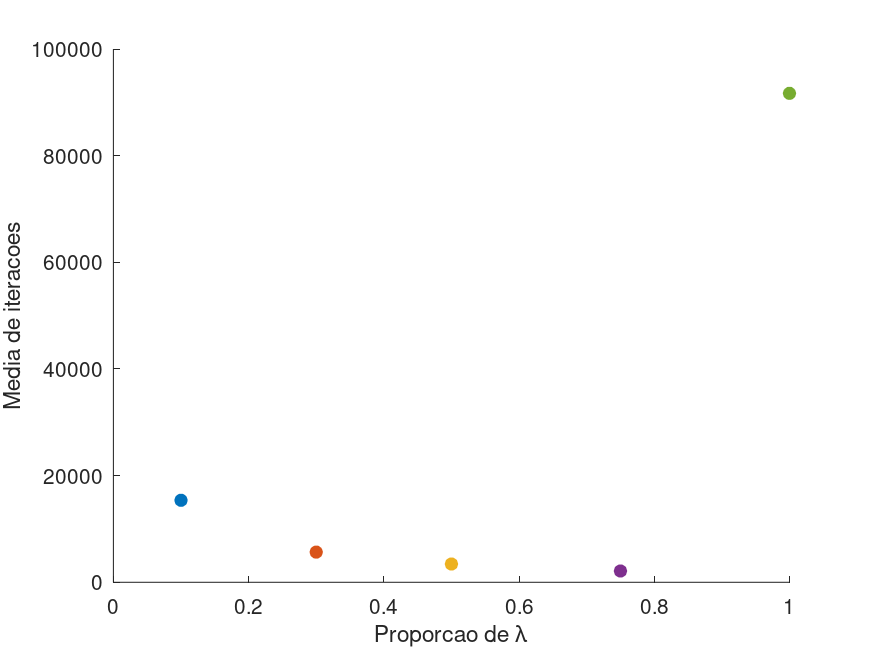
\includegraphics[scale=0.45]{grad1000.png}
  \caption{G = diag(1, 2000, . . . , 10000)}
\end{figure}
Como visto nas figuras acima, quanto maior o número de condição de $G$ (10, 100, 1000 e 10000 para cada item, respectivamente), mais iterações são necessárias universalmente. Contudo, o quanto cada método é afetado varia. Uma teoria para explicar tal fenômeno é que, como visto em aula, visto que o problema do método do gradiente com passo exato é, com matrizes com alto número de condição, as iterações ficarem "presas" entre duas retas com inclinação pequena entre si, ao mudar-se a proporção do passo exato, é obtido perturbação suficiente para "escapar" desse comportamento repetitivo. Contudo esse efeito de perturbação é contestado pelo tamanho do passo, ou seja, existe um balanço entre tamanho do passo e perturbação de comportamento ótimo; muita perturbação e um passo muito pequeno, como é o caso de $0.1\lambda$, e o método não é tão rápido, assim como, no extremo oposto, perturbação nula e passo grande, como é o caso de $\lambda$, não produz bons resultados também. Como visto nos gráficos acima, o valor ótimo dentre os fornecidos é $0.8\lambda$, que apresenta uma perturbação considerável de comportamento em comparação ao método com passo exato, porém com passos de tamanho significativo ainda. Isso sendo dito, é óbvio que o maior agravante para casos extremos ainda é a falta de perturbação do método do gradiente com passo exato, pois, apesar de começar melhor em performance do que $0.1\lambda$ e ter performance semelhante a $0.3\lambda$ no problema com $G = diag(1, 2, . . . , 10)$, $\lambda$ logo se mostra a pior alternativa com o aumento do número de condição, chegando a ser uma ordem de magnitude mais devagar que as demais proporções para $G = diag(1, 2000, . . . , 10000)$, se distanciando delas cada vez mais rápido.
\section{Exercício2}
\subsection{Preparativos}
O gradiente da função de Rosenbrock é dado por
\begin{equation}
\nabla f(x)=
\begin{pmatrix}
x_1+2x_1^3-2x_1x_2-1\\ 
x_2-x_1^2
\end{pmatrix}
\end{equation}
Sua Hessiana por
\begin{equation}
H_f(x)=
\begin{pmatrix}
2(x_1^2-x_2)+4x_1^2+1& -2x_1\\ 
-2x_1& 1
\end{pmatrix}
\end{equation}
E seu Laplaciano por
\begin{equation}
\nabla^2f(x)=6x_1^2-2x_2+2
\end{equation}
\subsection{Algoritmo do método do gradiente com Armijo}
O algoritmo é muito semelhante ao do Exercício 1 (para entender a obtenção de $x_0$ e o que são as variáveis inicializadas no algoritmo, refira-se a Seção 1.1), fazendo-se as mudanças necessárias para a nova função e com a atualização do iterando sendo levemente diferente.
Uma das mudanças é a inserção de funções para o cálculo do gradiente e da hessiana (como em (1) e (2)) e da própria $f(x)$, que anteriormente era trivial e feito diretamente na main. Algoritmo:
\begin{lstlisting}
function grad_x=gradiente(x)
    grad_x=[x(1)+2*x(1)^3-2*x(1)*x(2)-1; x(2)-x(1)^2];
endfunction
function hessian_x=hessian(x)
    hessian_x=[2*(x(1)^2-x(2))+4*x(1)^2+1, -2*x(1); -2*x(1), 1];
endfunction
f=@(x) ((x(1)^2-x(2))^2+(1-x(1))^2)/2;
\end{lstlisting}
A direção de descida ainda é menos o vetor gradiente, e por (1) e (2), o $\lambda$ do passo exato é dado por
\[
\lambda=-\frac{\nabla f(x_k)^Td_k}{d_k^TH_f(x_k)d_k}=-\frac{\nabla f(x_k)^T(-\nabla f(x_k))}{(-\nabla f(x_k))^TH_f(x_k)(-\nabla f(x_k))}=\frac{||\nabla f(x_k)||^2}{\nabla f(x_k)^TH_f(x_k)\nabla f(x_k)}
\]
Algoritmo:
\begin{lstlisting}
         lambda=normgrad/(transpose(grad)*hessian(xk)*grad);
\end{lstlisting}
Após a obtenção desse $\lambda$, será satisfeita a condição de Armijo-Goldstein. Equanto 
\[
f(x_k)-f(x_k+\lambda d_k)=f(x_k)-f(x_k-\lambda \nabla f(x_k))\geq -\lambda\alpha\nabla f(x_k)^Tdk=\lambda\alpha||\nabla f(x_k)||^2
\]
A variável $\lambda$ é atualizado como 0.8 vezes ela prórpria. Do enunciado, $\alpha=0.5$. Para economizar operações, $f(x_k)$, $x_k-\lambda\nabla f(x_k)$ e $\alpha||\nabla f(x_k)||^2$ são armazenados, pois possivelmente serão usados diversas vezes. Algoritmo:
\begin{lstlisting}
        f_xk=f(xk)
        alpha_normgrad=0.5*normgrad;
        xk1=xk-lambda*grad;
        while (f_xk-f(xk1)<=alpha_normgrad*lambda)
            lambda*=0.8;
            xk1=xk-lambda*grad;
        endwhile
        xk=xk1;                 
\end{lstlisting}
Como a convergência não é garantida para esse método nesse caso, outra mudança em comparação ao Exercício 1 é que uma condição secundária de parada foi introduzida; $\lambda$ ser menor que a precisão de máquina. Além disso, após o término das iterações, um \verb+if+ foi introduzido para averiguar o motivo do término; em caso de convergência à solução ótima (\verb+normgrad<=eps+), o número de iterações é contabilizado, e caso contrário (\verb+lambda<=eps+), é contabilizado na variável \verb+not_min+ mais um ponto inicial que não convergiu à solução ótima (informação usada na análise dos resultados, na Seção 2.4). Algoritmo:
\begin{lstlisting}
    do
        .
        .
        .
    until (normgrad<=eps || lambda<=eps)
    if (normgrad<=eps)
        iterations+=j;
    else
        not_min++;
    endif
endfor
\end{lstlisting}
Algoritmo completo:
\begin{lstlisting}
num_iter=10000;
function grad_x=gradiente(x)
    grad_x=[x(1)+2*x(1)^3-2*x(1)*x(2)-1; x(2)-x(1)^2];
endfunction
function hessian_x=hessian(x)
    hessian_x=[2*(x(1)^2-x(2))+4*x(1)^2+1, -2*x(1); -2*x(1), 1];
endfunction
f=@(x) ((x(1)^2-x(2))^2+(1-x(1))^2)/2;
iterations=0;
not_min=0;
for t=1:num_iter
    xk=rand(2,1);
    for i=1:2
        do
            aux=randi([-10,10]);
        until aux!=0
        xk(i)*=aux;
    endfor
    xk_0=xk;
    j=0;
    do 
        grad=gradiente(xk);
        normgrad=dot(grad,grad);
        lambda=normgrad/(transpose(grad)*hessian(xk)*grad);
        f_xk=f(xk);
        alpha_normgrad=0.5*normgrad;
        xk1=xk-lambda*grad;
        while (f_xk-f(xk1)<=alpha_normgrad*lambda)
            lambda*=0.8;
            xk1=xk-lambda*grad;
        endwhile
        xk=xk1;         
        j++;
    until (normgrad<=eps || lambda<=eps)
    if (normgrad<=eps)
        iterations+=j;
    else
        not_min++;
    endif
endfor
\end{lstlisting}
\subsection{Algoritmo do método de Newton}
O algoritmo é muito semelhante ao do exercício 2 (para entender a obtenção de $x_0$ e o que são as variáveis inicializadas no algoritmo, refira-se a Seção 2.2, fazendo-se as mudanças necessárias para a atualização do iterando pelo método de Newton).
Uma das mudanças é a inserção da função para o cálculo do Laplaciano de $f(x)$, como visto em (3), e que será usada nesse método. Algoritmo:
\begin{lstlisting}
function grad_x=gradiente(x)
    grad_x=[x(1)+2*x(1)^3-2*x(1)*x(2)-1; x(2)-x(1)^2];
endfunction
laplacian=@(x) 6*x(1)^2-2*x(2)+2;
f=@(x) ((x(1)^2-x(2))^2+(1-x(1))^2)/2;
\end{lstlisting}
A direção de descida ainda é menos o vetor gradiente, e por (1) e (3), o passo para Newton puro é dado por
\[
x_{k+1}=x_k-\frac{1}{\nabla^2 f(x_k)}\nabla f(x_k)
\]
Algoritmo:
\begin{lstlisting}
	  grad=gradiente(xk);
	  normgrad=dot(grad,grad);
	  xk-=grad/laplacian(xk);
\end{lstlisting}
Outra mudança em comparação ao Exercício 1 é que, pela falta de garantia de convergência à solução ótima para o método de Newton puro nesse caso, uma condição secundária de parada foi introduzida; o número de iterações seja igual a 10000 (número obtido experimentalmente). Algoritmo:
\begin{lstlisting}
    do
        .
        .
        .
    until (normgrad<=eps || j==10000)
\end{lstlisting}
 Algoritmo completo:
\begin{lstlisting}
num_iter=10000;
function grad_x=gradiente(x)
    grad_x=[x(1)+2*x(1)^3-2*x(1)*x(2)-1; x(2)-x(1)^2];
endfunction
laplacian=@(x) 6*x(1)^2-2*x(2)+2;
f=@(x) ((x(1)^2-x(2))^2+(1-x(1))^2)/2;
iterations=0;
not_min=0;
for t=1:num_iter
    xk=rand(2,1);
    for i=1:2
        do
            aux=randi([-10,10]);
        until aux!=0
        xk(i)*=aux;
    endfor
    xk_0=xk;
    j=0;
    do 
        grad=gradiente(xk);
        normgrad=dot(grad,grad);
        xk-=grad/laplacian(xk);           
        j++;
    until (normgrad<=eps || j==10000)
    if (normgrad<=eps)
        iterations+=j;
    else
        not_min++;
    endif    
endfor
\end{lstlisting}
\subsection{Resultados}
\begin{figure}[H]
  \centering
  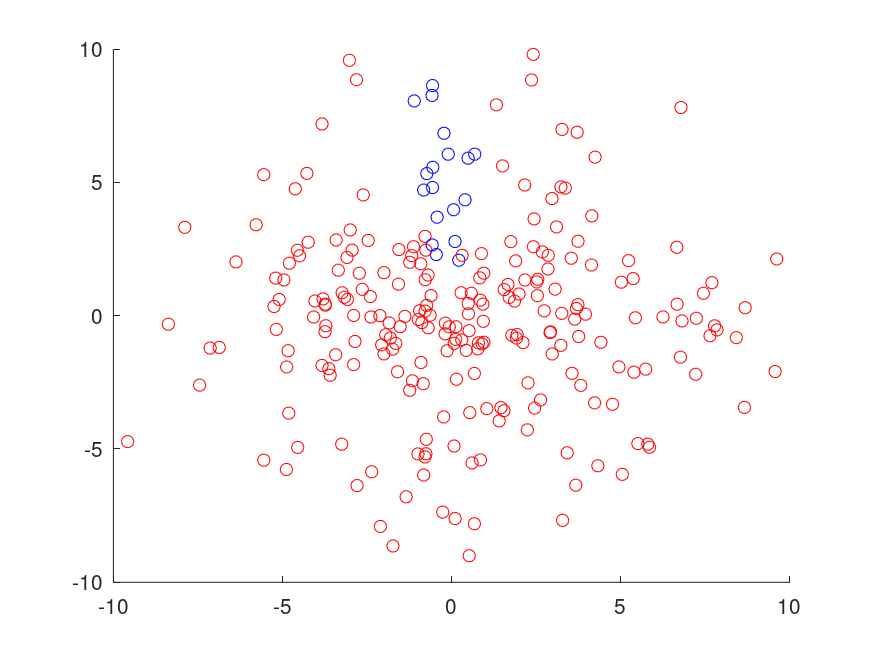
\includegraphics[scale=0.4]{newton}
  \caption{Comportamento do método de Newton puro para 250 pontos iniciais}
\end{figure}
No gráfico acima estão dispostos em azul os pontos iniciais ($x_0$) que não convergiram para a solução ótima, e em vermelho os que convergiram.
\begin{figure}[H]
  \centering
  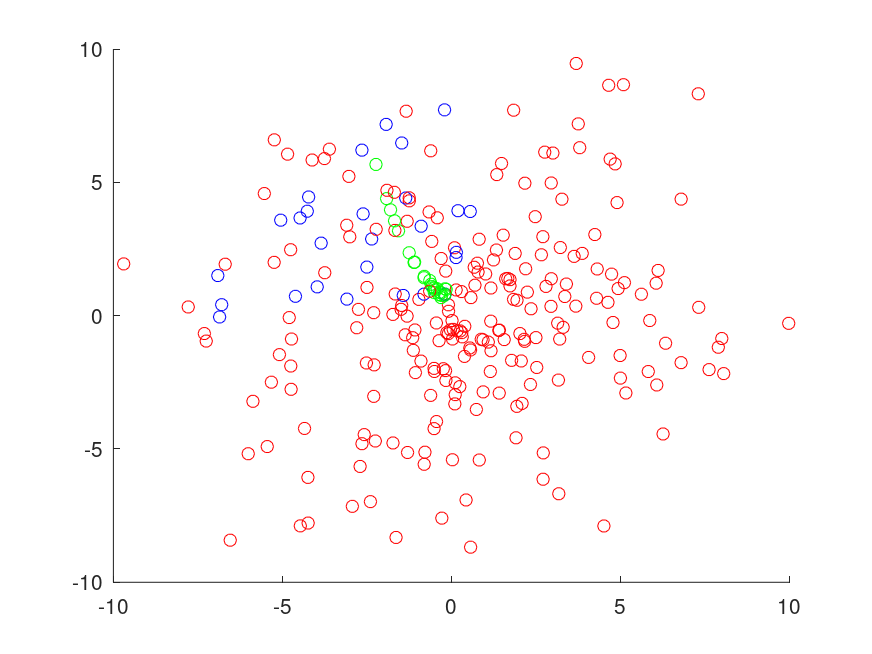
\includegraphics[scale=0.4]{armijo}
  \caption{Comportamento do método com Armijo para 250 pontos iniciais}
\end{figure}
O gráfico acima segue a mesma regra de coloração que o anterior, e adicionalmente em verde estão as iterações finais dos pontos que não convergiram para a solução ótima.

Além dos gráficos acima, cada método foi testado com 10000 pontos iniciais diferentes, com os resultados sendo
\begin{table}[H]
\centering
\begin{tabular}{|c||c|c|}
\hline&Média de iterações (arredondado)&Porcentagem de soluções não mínimas\\
\hline Armijo&81&11.81\%\\
\hline Newton&583&6.63\%\\
\hline
\end{tabular}
\caption{Resultados}
\end{table}
Na tabela acima, o número de iterações só leva em consideração pontos iniciais que convergiram para a solução ótima. Além disso, foi constatado que os pontos que não convergiram à solução ótima no método de Newton puro foram crescendo indeterminadamente na direção do eixo vertical (terminando aproximadamente em $(-10^{-4}, 5\cdot10^{3})^T$). É possível observar, da Figura 5, que o método de Newton não funciona para pontos iniciais próximos do eixo vertical positivo, que são levados à um máximo local. De fato, um dos problemas do método de Newton puro é a não garantia da direção escolhida ser de descida, como visto em aula. Já o método do gradiente com Armijo fica  preso em uma curva, observável pelos pontos verdes da Figura 6, com os pontos que são atraídos a tal vale estando no segundo quadrante sem muita concentração em uma região específica. No geral, com escolha randômica de ponto inicial, o método de Newton apresenta menor porcentagem de soluções indesejadas, como visto na Tabela 1. O problema é que, dado um ponto escolhido à mão, um viés de seleção é muito mais provável de causar não convergência no método de Newton que no do gradiente. Para entender o comportamento de ambos os métodos, foi efetuado um plot da função objetivo usando o programa Mathematica:
\begin{figure}[H]
  \centering
  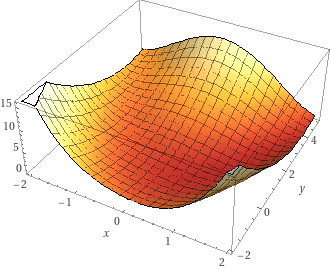
\includegraphics[scale=1]{curve}
  \caption{Plot da função objetivo}
\end{figure}
Como pode ser visto nas Figuras 6 e 7, o método do gradiente fica preso no vale no segundo quadrante, enquanto o método de Newton procura o máximo local no "morro" no eixo vertical positivo. Ambos os comportamentos, portanto, parecem coincidir com e ter uma uma explicação baseada na curvatura da função.

Fazendo a análise de $flops$ específicos para cada método, tem-se que o método de Newton apresenta 5 $flops$ do cálculo de Laplaceano e 2 $flops$ da divisão do vetor gradiente por esse Laplaceano, enquanto que o método do gradiente apresenta 8 $flops$ para o cálculo da Hessiana, 9 para efetuar $\nabla f(x_k)^TH_f(x_k)\nabla f(x_k)$, 1 para a divisão da norma do gradiente ao quadrado por esse valor, 6 para o cálculo de $f(x_k)$, 2 para a multiplicação do $\alpha\lambda||\nabla f(x_k)||$, 2 pelo cálculo de $\lambda\nabla f(x_k)$, e mais 6 pelo cálculo de $f(x_k-\lambda\nabla f(x_k))$, isso assumindo que $\lambda$ satisfaça a condição logo de início. Ou seja, comparando esses $flops$ específicos, tem-se que o método do gradiente apresenta 27 $flops$ a mais que o método de Newton no melhor caso possível. Os métodos apresentam 15 $flops$ em comum (cálculo do gradiente e de sua norma, além da soma do passo à $x_k$) no melhor caso possível, logo o método do gradiente apresenta $\frac{42}{15}$ mais $flops$ que seu concorrente. Contudo, cada atualização de $\lambda$ após a primeira de cada iteração custa 12 $flops$, logo são necessárias poucas atualizações do $\lambda$ para que a vantagem do método do gradiente em número de $flops$ (Tabela 1) seja negada. Entretanto, rodando cada algoritmo com 1000 pontos iniciais e contando o tempo necessário em condições constantes de processamento da máquina, foi constatado que o método do gradiente com Armijo é significativamente mais rápido (cerca de 12.2 s) que o de Newton puro (cerca de 89.2 s), garantindo com alta margem de segurança estatística que a performance do primeiro é melhor do que a do segundo para esse caso. Mesmo com maior porcentagem de soluções indesejadas, o método do gradiente com Armijo seria recomendável para esse problema, devido a sua performance superior.
\section{Referências Bibliográficas}
\begin{itemize}
\item Arenales, M.; Armentano, V. A.; Morabito, R.; Yanasse, H. H. \textbf{Pesquisa operacional}. Rio de Janeiro: Campus, 2007.
\item Bazaraa, M. Jarvis, J., Sherali, H. \textbf{Linear Programming and Network Flows}. John Wiley \& Sons, 1990.
\end{itemize}
\end{document}